% 2011 年北京卷理科第 5 题：圆 O 的两条切线与一条割线。
% 来源 PDF：普通高考/2011/2011北京理.pdf，SHA-256 79351b2b5d5afd29a2d46d50526284443edad4deb64fbaf841db31ce2570c311。
% 原页：第 1 页（A3 三栏）第 1 栏下部，书页码 647。
% 重绘依据：照原页拓扑——A 在圆外左下，AD、AE 为两条切线（切点 D 在下、E 在左上），
%   BC 为第三条切线（切点 F 在左下弧上），B 在线段 AD 上、C 在线段 AE 上；
%   割线 A—F 延长交圆于 G，G 在圆右侧；O 为圆心。不按比例。
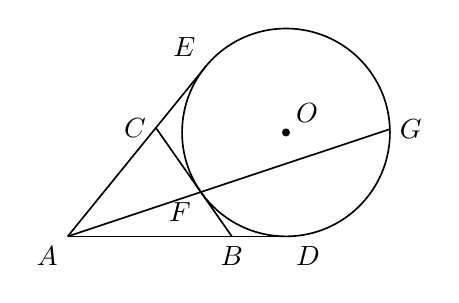
\begin{tikzpicture}[>=stealth, semithick, scale=1.32]
  \coordinate (O) at (0,0);
  \coordinate (A) at (-2.1,-1.0);
  \coordinate (B) at (-0.521,-1.0);
  \coordinate (C) at (-1.252,0.045);
  \coordinate (D) at (0,-1.0);
  \coordinate (E) at (-0.776,0.630);
  \coordinate (F) at (-0.819,-0.574);
  \coordinate (G) at (0.999,0.032);

  \draw (O) circle (1);

  % 两条切线 AD、AE
  \draw (A) -- (D);
  \draw (A) -- (E);
  % 第三条切线 BC
  \draw (B) -- (C);
  % 割线 A—F—G
  \draw (A) -- (G);

  % 字母标号
  \node[below left] at (A) {$A$};
  \node[below] at (B) {$B$};
  \node[left] at (C) {$C$};
  \node[below right] at (D) {$D$};
  \node[above left] at (E) {$E$};
  \node[below left] at (F) {$F$};
  \node[right] at (G) {$G$};

  % 圆心 O
  \fill (O) circle (1.1pt);
  \node[above right] at (O) {$O$};
\end{tikzpicture}
